
\section*{CHƯƠNG 2. PHÂN TÍCH HỆ THỐNG}
\setcounter{section}{2}
\setcounter{subsection}{0} %LƯU Ý MỖI LẦN THÊM CHƯƠNG MỚI CẦN THÊM CÂU NÀY ĐỂ RESET THỨ TỰ CỦA SUBSECTON VỀ 1
\setcounter{table}{0} % LƯU Ý SAU MỖI LẦN GỌI BẢNG HAY HÌNH ẢNH PHẢI THÊM CÂU NÀY ĐỂ RESET THỨ TỰ
\setcounter{figure}{0} %% LƯU Ý SAU MỖI LẦN GỌI BẢNG HAY HÌNH ẢNH PHẢI THÊM CÂU NÀY ĐỂ RESET THỨ TỰ
\addcontentsline{toc}{section}{\numberline{}CHƯƠNG 2. PHÂN TÍCH HỆ THỐNG}
Trong chương này, chúng em sẽ tiến hành phân tích hệ thống cho dự án đề tài "Hệ thống theo dõi và quản lý dữ liệu điện tim" dựa trên các mục tiêu
đã nêu ra trong Mục Đề xuất hệ thống ở Phần mở đầu. Trước tiên bài toán đặt ra ở hệ thống là:
\begin{adjustwidth}{1.5em}{}
\begin{itemize}
  \item Một ứng dụng để có thể giúp người dùng/bệnh nhân theo dõi được những thông tin cần về sức khoẻ tim mạch
  \item Trực quan và tiêu chuẩn hoá những thông tin đo được
    bằng hình ảnh hoặc số liệu để bác sĩ có thể dựa vào đó để đưa ra những đánh giá cho người dùng. Ngoài ra những thông tin này
    có thể hữu ích trong việc theo dõi sức khỏe tim mạch, theo dõi hiệu quả của liệu pháp 
    và hỗ trợ quyết định của người dùng
  \item Quản trị viên sẽ là người có thể phân công bác sĩ để chăm sóc, theo dõi sức khoẻ từ
  xa cho bệnh nhân
\end{itemize}
\end{adjustwidth}
Chi tiết về việc phân tích các yêu cầu hệ thống sẽ được chúng em trình bày ở các chương dưới.

\subsection{Sơ đồ use case}
\subsubsection{Use case tổng quát hệ thống}
Dựa vào những phân tích về yêu cầu chức năng, các use case trong hệ thống được chúng em thể hiện ở hình dưới 
  \begin{figure}[H]
    \centering
    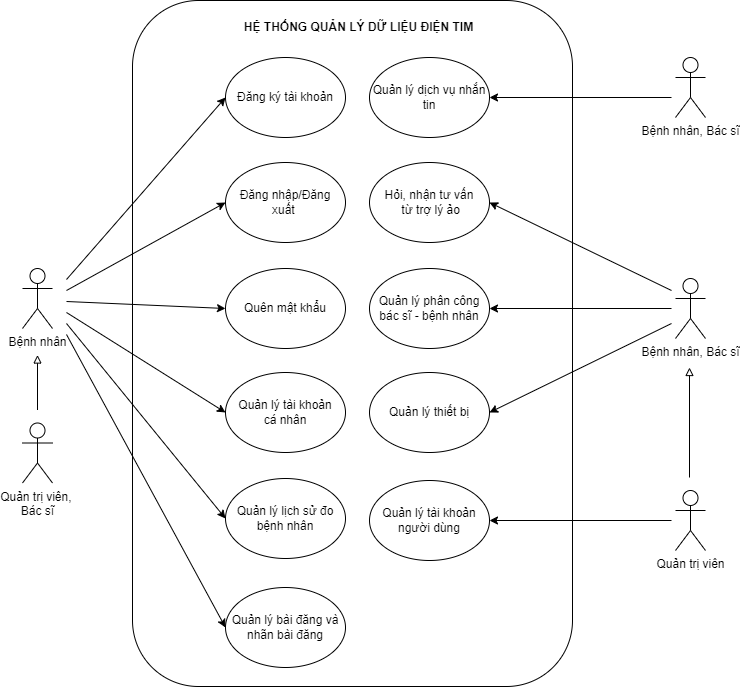
\includegraphics[width=16cm,height=14cm]{Images/use_case/use_case_general.png}
    \caption[Sơ đồ use case tổng quát của hệ thống]{\bfseries \fontsize{12pt}{0pt}
    \selectfont Sơ đồ use case tổng quát của hệ thống}
    \label{use_case_general} %đặt tên cho ảnh
  \end{figure}

\subsubsection{Use case chức năng đăng ký tài khoản}
  \begin{figure}[H]
    \centering
    \caption[Sơ đồ use case chức năng đăng ký tài khoản]{\bfseries \fontsize{12pt}{0pt}
    \selectfont Sơ đồ use case chức năng đăng ký tài khoản}
    \label{use_case_register} %đặt tên cho ảnh
  \end{figure}

  \begin{table}[H]
    \caption{\bfseries \fontsize{12pt}{0pt}\selectfont Bảng phân tích use case chức năng đăng ký tài khoản}
    \centering
    \begin{tabularx}{0.9\textwidth}{|c|X|}
      \hline
      \textbf{Tên chức năng} & \textbf{Đăng ký tài khoản} \\
      \hline
      Tác nhân & Bệnh nhân, Bác sĩ, Quản trị viên \\
      \hline
      Mô tả & Cho phép người dùng đăng ký tài khoản để truy cập vào các tài nguyên của hệ thống 
       \\
      \hline
      Điều kiện trước & Người dùng cần có kết nối Internet \\
      \hline
      Dòng sự kiện chính & 
      % \begin{tabular}{@{}l@{}}
        Chi tiết luồng sự kiện được thể hiện ở Hình \ref{}, Hình \ref{} 
        \\
      % \end{tabular} \\
      \hline
    \end{tabularx}
  \end{table}

\subsubsection{Use case chức năng đăng nhập/đăng xuất }
  \begin{figure}[H]
    \centering
    \caption[Sơ đồ use case chức năng đăng nhập/đăng xuất]{\bfseries \fontsize{12pt}{0pt}
    \selectfont Sơ đồ use case chức năng đăng nhập/đăng xuất}
    \label{use_case_login_logout} %đặt tên cho ảnh
  \end{figure}

  \begin{table}[H]
    \caption{\bfseries \fontsize{12pt}{0pt}\selectfont Bảng phân tích use case chức năng đăng nhập/đăng xuất}
    \centering
    \begin{tabularx}{0.9\textwidth}{|c|X|}
      \hline
      \textbf{Tên chức năng} & \textbf{Đăng nhập/Đăng xuất} \\
      \hline
      Tác nhân & Bệnh nhân, Bác sĩ, Quản trị viên \\
      \hline
      Mô tả & Cho phép người dùng sử dụng tài khoản để truy cập vào các tài nguyên của hệ thống và có thể đăng xuất hệ thống
       \\
      \hline
      Điều kiện trước & Người dùng cần có kết nối Internet \\
      \hline
      Dòng sự kiện chính & 
      % \begin{tabular}{@{}l@{}}
        Chi tiết luồng sự kiện được thể hiện ở Hình \ref{}, Hình \ref{} 
        \\
      % \end{tabular} \\
      \hline
    \end{tabularx}
  \end{table}

\subsubsection{Use case chức năng quên mật khẩu}
  \begin{figure}[H]
    \centering
    \caption[Sơ đồ use case chức năng quên mật khẩu]{\bfseries \fontsize{12pt}{0pt}
    \selectfont Sơ đồ use case chức năng quên mật khẩu}
    \label{use_case_forget_password} %đặt tên cho ảnh
  \end{figure}

  \begin{table}[H]
    \caption{\bfseries \fontsize{12pt}{0pt}\selectfont Bảng phân tích use case chức năng quên mật khẩu}
    \centering
    \begin{tabularx}{0.9\textwidth}{|c|X|}
      \hline
      \textbf{Tên chức năng} & \textbf{Quên mật khẩu} \\
      \hline
      Tác nhân & Bệnh nhân, Bác sĩ, Quản trị viên \\
      \hline
      Mô tả & Cho phép người dùng lấy lại mật khẩu tài khoản thông qua email
       \\
      \hline
      Điều kiện trước & Người dùng cần có kết nối Internet và truy cập vào email đăng ký \\
      \hline
      Dòng sự kiện chính & 
      % \begin{tabular}{@{}l@{}}
        Chi tiết luồng sự kiện được thể hiện ở Hình \ref{}, Hình \ref{} 
        \\
      % \end{tabular} \\
      \hline
    \end{tabularx}
  \end{table}

  \subsubsection{Use case chức năng quản lý tài khoản cá nhân}
  \begin{figure}[H]
    \centering
    \caption[Sơ đồ use case chức năng quản lý tài khoản cá nhân]{\bfseries \fontsize{12pt}{0pt}
    \selectfont Sơ đồ use case chức năng quản lý tài khoản cá nhân}
    \label{use_case_forget_password} %đặt tên cho ảnh
  \end{figure}

  \begin{table}[H]
    \caption{\bfseries \fontsize{12pt}{0pt}\selectfont Bảng phân tích use case chức năng quản lý tài khoản cá nhân}
    \centering
    \begin{tabularx}{0.9\textwidth}{|c|X|}
      \hline
      \textbf{Tên chức năng} & \textbf{Quản lý tài khoản cá nhân} \\
      \hline
      Tác nhân & Bệnh nhân, Bác sĩ, Quản trị viên \\
      \hline
      Mô tả & Cho phép người dùng xem, thay đổi thông tin cá nhân như số điện thoại, email, tên hiển thị
       \\
      \hline
      Điều kiện trước & Người dùng cần có kết nối Internet và đăng nhập \\
      \hline
      Dòng sự kiện chính & 
      % \begin{tabular}{@{}l@{}}
        Chi tiết luồng sự kiện được thể hiện ở Hình \ref{}, Hình \ref{} 
        \\
      % \end{tabular} \\
      \hline
    \end{tabularx}
  \end{table}

\subsubsection{Use case chức năng xem lịch sử các lần đo}
  \begin{figure}[H]
    \centering
    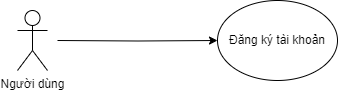
\includegraphics[width=9cm,height=2.5cm]{Images/use_case/use_case_register.png}
    \caption[Sơ đồ use case chức năng đăng ký tài khoản]{\bfseries \fontsize{12pt}{0pt}
    \selectfont Sơ đồ use case chức năng đăng ký tài khoản}
    \label{use_case_register} %đặt tên cho ảnh
  \end{figure}

  \begin{table}[H]
    \caption{\bfseries \fontsize{12pt}{0pt}\selectfont Bảng phân tích use case chức năng đăng ký tài khoản}
    \centering
    \begin{tabularx}{0.9\textwidth}{|c|X|}
      \hline
      \textbf{Tên chức năng} & \textbf{Đăng ký tài khoản} \\
      \hline
      Tác nhân & Bệnh nhân, Bác sĩ, Quản trị viên \\
      \hline
      Mô tả & Cho phép người dùng đăng ký tài khoản để truy cập vào các tài nguyên của hệ thống 
       \\
      \hline
      Điều kiện trước & Người dùng cần có kết nối Internet \\
      \hline
      Dòng sự kiện chính & 
      % \begin{tabular}{@{}l@{}}
        Chi tiết luồng sự kiện được thể hiện ở Hình \ref{}, Hình \ref{} 
        \\
      % \end{tabular} \\
      \hline
    \end{tabularx}
  \end{table}

\subsubsection{Use case chức năng đăng nhập/đăng xuất }
  \begin{figure}[H]
    \centering
    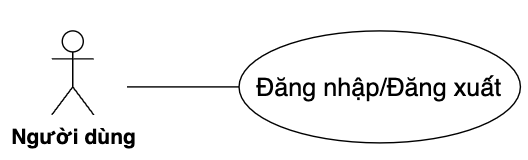
\includegraphics[width=9cm,height=2.5cm]{Images/use_case/use_case_login.png}
    \caption[Sơ đồ use case chức năng đăng nhập/đăng xuất]{\bfseries \fontsize{12pt}{0pt}
    \selectfont Sơ đồ use case chức năng đăng nhập/đăng xuất}
    \label{use_case_login_logout} %đặt tên cho ảnh
  \end{figure}

  \begin{table}[H]
    \caption{\bfseries \fontsize{12pt}{0pt}\selectfont Bảng phân tích use case chức năng đăng nhập/đăng xuất}
    \centering
    \begin{tabularx}{0.9\textwidth}{|c|X|}
      \hline
      \textbf{Tên chức năng} & \textbf{Đăng nhập/Đăng xuất} \\
      \hline
      Tác nhân & Bệnh nhân, Bác sĩ, Quản trị viên \\
      \hline
      Mô tả & Cho phép người dùng sử dụng tài khoản để truy cập vào các tài nguyên của hệ thống và có thể đăng xuất hệ thống
       \\
      \hline
      Điều kiện trước & Người dùng cần có kết nối Internet \\
      \hline
      Dòng sự kiện chính & 
      % \begin{tabular}{@{}l@{}}
        Chi tiết luồng sự kiện được thể hiện ở Hình \ref{}, Hình \ref{} 
        \\
      % \end{tabular} \\
      \hline
    \end{tabularx}
  \end{table}

\subsubsection{Use case chức năng quên mật khẩu}
  \begin{figure}[H]
    \centering
    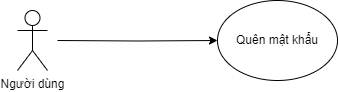
\includegraphics[width=9cm,height=2.5cm]{Images/use_case/use_case_forgot_password.png}
    \caption[Sơ đồ use case chức năng quên mật khẩu]{\bfseries \fontsize{12pt}{0pt}
    \selectfont Sơ đồ use case chức năng quên mật khẩu}
    \label{use_case_forget_password} %đặt tên cho ảnh
  \end{figure}

  \begin{table}[H]
    \caption{\bfseries \fontsize{12pt}{0pt}\selectfont Bảng phân tích use case chức năng quên mật khẩu}
    \centering
    \begin{tabularx}{0.9\textwidth}{|c|X|}
      \hline
      \textbf{Tên chức năng} & \textbf{Quên mật khẩu} \\
      \hline
      Tác nhân & Bệnh nhân, Bác sĩ, Quản trị viên \\
      \hline
      Mô tả & Cho phép người dùng lấy lại mật khẩu tài khoản thông qua email
       \\
      \hline
      Điều kiện trước & Người dùng cần có kết nối Internet và truy cập vào email đăng ký \\
      \hline
      Dòng sự kiện chính & 
      % \begin{tabular}{@{}l@{}}
        Chi tiết luồng sự kiện được thể hiện ở Hình \ref{}, Hình \ref{} 
        \\
      % \end{tabular} \\
      \hline
    \end{tabularx}
  \end{table}

\subsubsection{Use case chức năng quản lý tài khoản cá nhân}
  \begin{figure}[H]
    \centering
    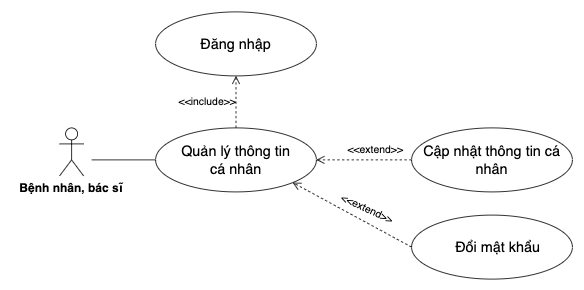
\includegraphics[width=14.8cm,height=9cm]{Images/use_case/use_case_manage_info.png}
    \caption[Sơ đồ use case chức năng quản lý tài khoản cá nhân]{\bfseries \fontsize{12pt}{0pt}
    \selectfont Sơ đồ use case chức năng quản lý tài khoản cá nhân}
    \label{use_case_manage_info} %đặt tên cho ảnh
  \end{figure}

  \begin{table}[H]
    \caption{\bfseries \fontsize{12pt}{0pt}\selectfont Bảng phân tích use case chức năng quản lý tài khoản cá nhân}
    \centering
    \begin{tabularx}{0.9\textwidth}{|c|X|}
      \hline
      \textbf{Tên chức năng} & \textbf{Quản lý tài khoản cá nhân} \\
      \hline
      Tác nhân & Bệnh nhân, Bác sĩ, Quản trị viên \\
      \hline
      Mô tả & Cho phép người dùng xem, thay đổi thông tin cá nhân như số điện thoại, email, tên hiển thị
       \\
      \hline
      Điều kiện trước & Người dùng cần có kết nối Internet và đăng nhập \\
      \hline
      Dòng sự kiện chính & 
      % \begin{tabular}{@{}l@{}}
        Chi tiết luồng sự kiện được thể hiện ở Hình \ref{}, Hình \ref{} 
        \\
      % \end{tabular} \\
      \hline
    \end{tabularx}
  \end{table}

\subsubsection{Use case chức năng quản lý dữ liệu đo}
  \begin{figure}[H]
    \centering
    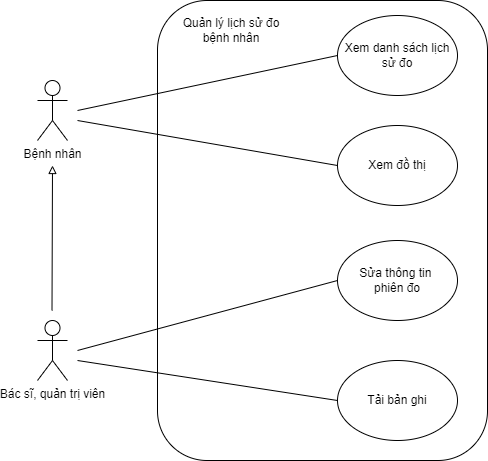
\includegraphics[width=15.2cm,height=9cm]{Images/use_case/use_case_view_history_record.png}
    \caption[Sơ đồ use case chức năng quản lý dữ liệu đo]{\bfseries \fontsize{12pt}{0pt}
    \selectfont Sơ đồ use case chức năng quản lý dữ liệu đo}
    \label{use_case_view_history_record} %đặt tên cho ảnh
  \end{figure}

  \begin{table}[H]
    \caption{\bfseries \fontsize{12pt}{0pt}\selectfont Bảng phân tích use case chức năng quản lý dữ liệu đo}
    \centering
    \begin{tabularx}{0.9\textwidth}{|c|X|}
      \hline
      \textbf{Tên chức năng} & \textbf{Xem lịch sử các lần đo} \\
      \hline
      Tác nhân & Bệnh nhân, Bác sĩ \\
      \hline
      Mô tả & Cho phép bệnh nhân xem lịch sử các lần đo điện tim, bác sĩ xem được lịch sử các lần đo, đồ thị của bệnh nhân
      mà mình quản lý.\\
      \hline
      Điều kiện trước & Người dùng cần có kết nối Internet và đã đăng nhập \\
      \hline
      Dòng sự kiện chính & 
      % \begin{tabular}{@{}l@{}}
        Chi tiết luồng sự kiện được thể hiện ở Hình \ref{view_record_timeline}, Hình \ref{getEcgRecordsByUserId}, Hình \ref{getEcgRecordsByDoctor} 
        \\
      % \end{tabular} \\
      \hline
    \end{tabularx}
  \end{table}

\subsubsection{Use case chức năng quản lí dịch vụ nhắn tin}
  \begin{figure}[H]
    \centering
    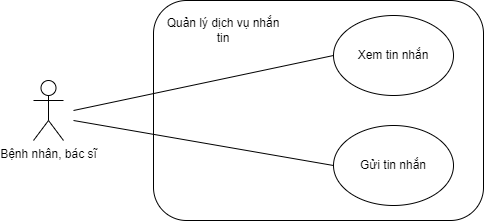
\includegraphics[width=14.7cm,height=8cm]{Images/use_case/use_case_send_receive_message.png}
    \caption[Sơ đồ use case chức năng quản lí dịch vụ nhắn tin]{\bfseries \fontsize{12pt}{0pt}
    \selectfont Sơ đồ use case chức năng quản lí dịch vụ nhắn tin}
    \label{use_case_chat} %đặt tên cho ảnh
  \end{figure}

  \begin{table}[H]
    \caption{\bfseries \fontsize{12pt}{0pt}\selectfont Bảng phân tích use case chức năng quản lí dịch vụ nhắn tin}
    \centering
    \begin{tabularx}{0.9\textwidth}{|c|X|}
      \hline
      \textbf{Tên chức năng} & \textbf{Quản lí dịch vụ nhắn tin} \\
      \hline
      Tác nhân & Bệnh nhân, Bác sĩ \\
      \hline
      Mô tả & Cho phép bệnh nhân chat với bác sĩ phụ trách và bác sĩ có thể chat với bệnh nhân mà mình phụ trách \\
      \hline
      Điều kiện trước & Người dùng cần có kết nối Internet và đã đăng nhập \\
      \hline
      Dòng sự kiện chính & 
      % \begin{tabular}{@{}l@{}}
        Chi tiết luồng sự kiện được thể hiện ở Hình \ref{}, Hình \ref{} 
        \\
      % \end{tabular} \\
      \hline
    \end{tabularx}
  \end{table}

\subsubsection{Use case chức năng tư vấn từ trợ lý ảo}
  \begin{figure}[H]
    \centering
    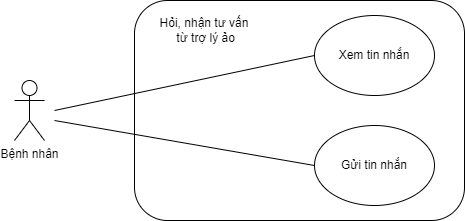
\includegraphics[width=12.5cm,height=5.8cm]{Images/use_case/use_case_chatbot.png}
    \caption[Sơ đồ use case chức năng tư vấn từ trợ lý ảo]{\bfseries \fontsize{12pt}{0pt}
    \selectfont Sơ đồ use case chức năng tư vấn từ trợ lý ảo}
    \label{use_case_chat_with_bot} %đặt tên cho ảnh
  \end{figure}

  \begin{table}[H]
    \caption{\bfseries \fontsize{12pt}{0pt}\selectfont Bảng phân tích use case chức năng tư vấn từ trợ lý ảo}
    \centering
    \begin{tabularx}{0.9\textwidth}{|c|X|}
      \hline
      \textbf{Tên chức năng} & \textbf{Tư vấn từ trợ lý ảo} \\
      \hline
      Tác nhân & Bệnh nhân \\
      \hline
      Mô tả & Cho phép bệnh nhân chat với chat bot trợ lý ảo \\
      \hline
      Điều kiện trước & Người dùng cần có kết nối Internet và đã đăng nhập \\
      \hline
      Dòng sự kiện chính & 
      % \begin{tabular}{@{}l@{}}
        Chi tiết luồng sự kiện được thể hiện ở Hình \ref{}, Hình \ref{} 
        \\
      % \end{tabular} \\
      \hline
    \end{tabularx}
  \end{table}  

\subsubsection{Use case chức năng quản lý bệnh nhân}
  \begin{figure}[H]
    \centering
    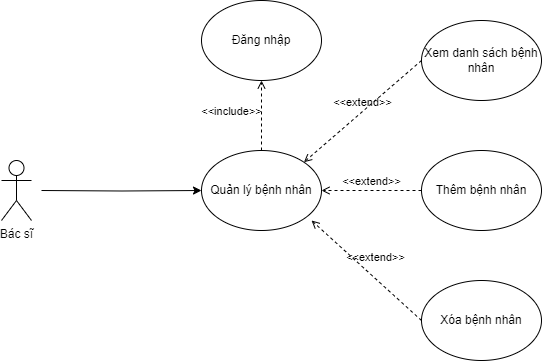
\includegraphics[width=14.2cm,height=8.5cm]{Images/use_case/use_case_manage_patients.png}
    \caption[Sơ đồ use case chức năng quản lý bệnh nhân]{\bfseries \fontsize{12pt}{0pt}
    \selectfont Sơ đồ use case chức năng quản lý bệnh nhân}
    \label{use_case_patient_management} %đặt tên cho ảnh
  \end{figure}

  \begin{table}[H]
    \caption{\bfseries \fontsize{12pt}{0pt}\selectfont Bảng phân tích use case chức năng quản lý bệnh nhân}
    \centering
    \begin{tabularx}{0.9\textwidth}{|c|X|}
      \hline
      \textbf{Tên chức năng} & \textbf{Quản lý bệnh nhân} \\
      \hline
      Tác nhân & Bác sĩ \\
      \hline
      Mô tả & Cho phép bác sĩ thực hiện hành động thêm, xóa bệnh nhân trong danh sách bệnh nhân của mình \\
      \hline
      Điều kiện trước & Người dùng cần có kết nối Internet và đã đăng nhập \\
      \hline
      Dòng sự kiện chính & 
      % \begin{tabular}{@{}l@{}}
        Chi tiết luồng sự kiện được thể hiện ở Hình \ref{}, Hình \ref{} 
        \\
      % \end{tabular} \\
      \hline
    \end{tabularx}
  \end{table}

\subsubsection{Use case chức năng quản lý thiết bị}
  \begin{figure}[H]
    \centering
    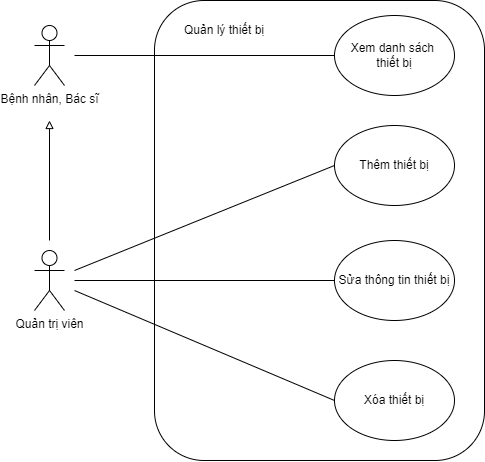
\includegraphics[width=14.2cm,height=9cm]{Images/use_case/use_case_manage_device.png}
    \caption[Sơ đồ use case chức năng quản lý thiết bị]{\bfseries \fontsize{12pt}{0pt}
    \selectfont Sơ đồ use case chức năng quản lý thiết bị}
    \label{use_case_device_management} %đặt tên cho ảnh
  \end{figure}

  \begin{table}[H]
    \caption{\bfseries \fontsize{12pt}{0pt}\selectfont Bảng phân tích use case chức năng quản lý thiết bị}
    \centering
    \begin{tabularx}{0.9\textwidth}{|c|X|}
      \hline
      \textbf{Tên chức năng} & \textbf{Quản lý thiết bị} \\
      \hline
      Tác nhân & Quản trị viên \\
      \hline
      Mô tả & Cho phép quản trị thực hiện hành động thêm, sửa, xóa các thiết bị, có thể xem đồ thị bản ghi thiết bị cũng như
      xuất ra định dạng file \\
      \hline
      Điều kiện trước & Người dùng cần có kết nối Internet và đã đăng nhập \\
      \hline
      Dòng sự kiện chính & 
      % \begin{tabular}{@{}l@{}}
        Chi tiết luồng sự kiện được thể hiện ở Hình \ref{}, Hình \ref{} 
        \\
      % \end{tabular} \\
      \hline
    \end{tabularx}
  \end{table}

\subsubsection{Use case chức năng quản lý tài khoản người dùng}
  \begin{figure}[H]
    \centering
    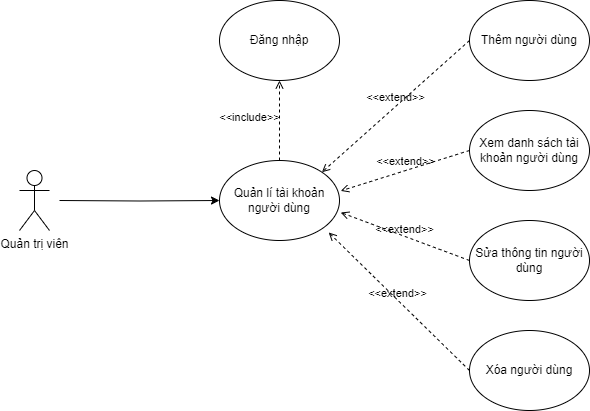
\includegraphics[width=15cm,height=10.5cm]{Images/use_case/use_case_manage_users.png}
    \caption[Sơ đồ use case chức năng tài khoản người dùng]{\bfseries \fontsize{12pt}{0pt}
    \selectfont Sơ đồ use case chức năng tài khoản người dùng}
    \label{use_case_user_management} %đặt tên cho ảnh
  \end{figure}

  \begin{table}[H]
    \caption{\bfseries \fontsize{12pt}{0pt}\selectfont Bảng phân tích use case chức năng quản lý thiết bị}
    \centering
    \begin{tabularx}{0.9\textwidth}{|c|X|}
      \hline
      \textbf{Tên chức năng} & \textbf{Quản lý tài khoản người dùng} \\
      \hline
      Tác nhân & Quản trị viên \\
      \hline
      Mô tả & Cho phép quản trị thực hiện hành động thêm, sửa, xóa đối với tài khoản người dùng \\
      \hline
      Điều kiện trước & Người dùng cần có kết nối Internet và đã đăng nhập \\
      \hline
      Dòng sự kiện chính & 
      % \begin{tabular}{@{}l@{}}
        Chi tiết luồng sự kiện được thể hiện ở Hình \ref{}, Hình \ref{} 
        \\
      % \end{tabular} \\
      \hline
    \end{tabularx}
  \end{table}

% \newpage
\subsection{Thẻ CRC (Class - Responsibility - Collaboration Card)}

\subsubsection{Thẻ CRC lớp User}
  \begin{table}[H]
    \caption{\bfseries \fontsize{12pt}{0pt}\selectfont Thẻ CRC lớp User}
    \centering
    \begin{tabularx}{0.9\textwidth}{X}
      Mặt trước thẻ
    \end{tabularx}
    \begin{tabularx}{0.9\textwidth}{|X|X|X|}
      \hline
      \textbf{Class name:} User & \textbf{ID:} 1 & \textbf{Type:} Concrete, Domain \\
      \hline
    \end{tabularx}
    \begin{tabularx}{0.9\textwidth}{|X|X|}
      \textbf{Description:} Đối tượng mô tả thông tin người dùng & \textbf{Associated use case:} 2 \\
      \hline
      \textbf{Responsibility:} & \textbf{Collaboration:} \\
      Thông tin nhân viên & Device \\
      \hline
    \end{tabularx}
    \begin{tabularx}{0.9\textwidth}{X}
      Mặt sau thẻ
    \end{tabularx}
    \begin{tabularx}{0.9\textwidth}{|X|X|}
      \hline
      \textbf{Attributes} & \\
      id(String) & image(String) \\
      accountId(String) & role(Int) \\
      username(String) & createdAt(BigInt) \\
      birth(BigInt) & updatedAt(BigInt) \\
      phoneNumber(String) & \\
      \hline
    \end{tabularx}
    \begin{tabularx}{0.9\textwidth}{|X|}
      \textbf{Relationships} \\
      Generalize:  \\
      Aggregation:  \\
      Association:  \\
      \hline
    \end{tabularx}
  \end{table}
% \newpage
\subsection{Sơ đồ lớp}

% \newpage
\subsection{Sơ đồ tuần tự}

\subsection{Phân tích dữ liệu}

Tại phần này, chúng em sẽ tiến hành xác định và mô tả các thực thể cũng như
 thuộc tính quan trọng trong hệ thống. Việc này giúp chúng ta có cái
  nhìn tổng quan về các yếu tố chính cần được quản lý và lưu trữ
   trong cơ sở dữ liệu. Bằng cách làm điều này, chúng ta có thể
    xây dựng một mô hình dữ liệu cơ bản để hỗ trợ việc thiết kế và
     triển khai hệ thống một cách hiệu quả.

     Trước hết, chúng em sẽ xác định và mô tả các thực thể chính trong hệ
      thống. Thực thể là các đối tượng hoặc khái niệm quan
       trọng mà chúng ta cần theo dõi và quản lý. Sau đó, chúng ta sẽ xác
        định các thuộc tính liên quan đến mỗi thực thể, các thông tin cần
         được lưu trữ và quản lý.

\begin{table}[H]
  \caption{\bfseries \fontsize{12pt}{0pt}\selectfont Bảng thực thể và thuộc tính}
  \centering
  \begin{tabularx}{0.9\textwidth}{|c|X|}
    \hline
    \textbf{Thực thể} & \textbf{Thuộc tính} \\
    \hline
    Người dùng & 
    ID người dùng, ID tài khoản, Tên người dùng, Email, Mật khẩu, Ngày sinh, Giới tính, Số điện thoại, Quyền, Thông tin người dùng \\
    \hline
    Token đăng nhập &
    ID token, ID tài khoản, Token truy cập, Token làm mới \\
    \hline
    Thiết bị & 
    ID thiết bị, ID người dùng thiết bị, ID bác sĩ theo dõi, Tên thiết bị, Loại thiết bị, Thông tin thiết bị, Trạng thái thiết bị, Ngày bắt đầu sử dụng\\
    \hline
    Các tần số đo được của thiết bị &
    ID tần số, ID thiết bị, Tên loại tần số, Thông tin, Giá trị đo được \\
    \hline
    Bản ghi ECG & 
    ID bản ghi ECG, ID người dùng, ID thiết bị, Loại bản ghi, Đường dẫn lưu trữ dữ liệu, Thời gian bắt đầu đo, Thời gian kết thúc đo \\
    \hline
    Thông tin hội thoại &
    ID hội thoại, ID người dùng tham gia \\
    \hline
    Tin nhắn & 
    ID tin nhắn, ID hội thoại, ID người gửi, ID người nhận, Nội dung tin nhắn, Thời gian gửi \\
    \hline
    Phân công bệnh nhân - bác sĩ & 
    ID phân công, ID bệnh nhân, ID bác sĩ, Ngày bắt đầu, Ngày kết thúc \\
    \hline
  \end{tabularx}

  
\end{table}
Sau khi hoàn thành được bảng thực thể và thuộc tính, chúng em xác định được mô hình thực thể liên kết như sau:

\begin{figure}[H]
  \centering
  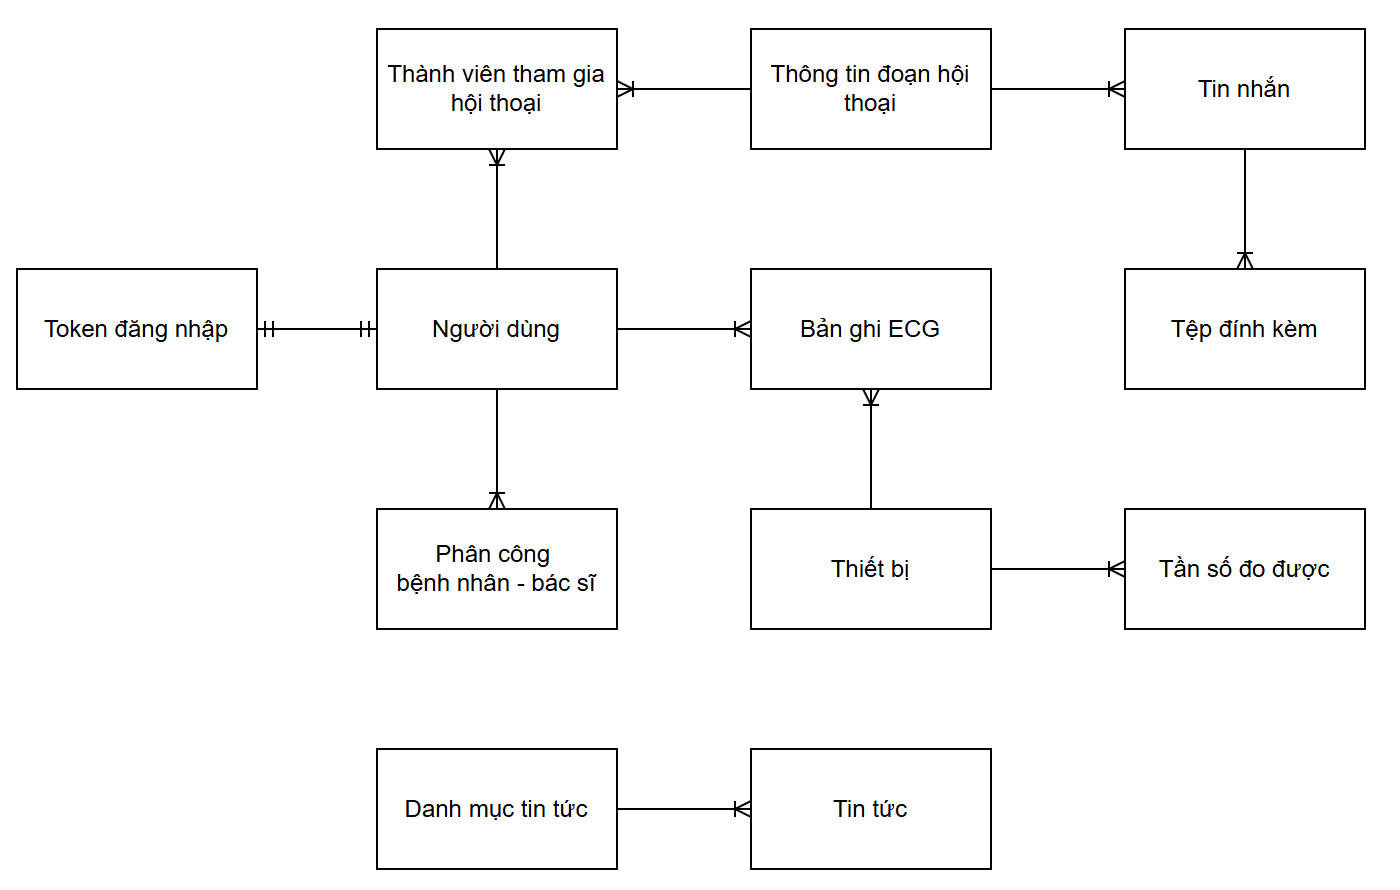
\includegraphics[width=15cm,height=8cm]{Images/system/fmECG_connection_entity.png}
  \caption[Mô hình thực thể liên kết]{\bfseries \fontsize{12pt}{0pt}
  \selectfont Mô hình thực thể liên kết}
  \label{ttlk} %đặt tên cho ảnh
\end{figure}


\subsection{Kết luận chương}

Trong chương này, chúng em đã thực hiện phân tích toàn diện về
 hệ thống cho đề tài , nhằm đáp ứng
  các mục tiêu và yêu cầu đã được đề xuất.

Chúng em đã xác định rõ ràng các khía cạnh quan trọng của hệ thống,
 tập trung vào việc thiết kế một hệ thống quản lý ECG hiệu quả,
  trực quan và có khả năng theo dõi sức khỏe tim mạch một cách
   chính xác. 


\newpage
